
\begin{frame}{The Internet}
    \begin{itemize}
    \item Perhaps the most successful computer application ever
    \item Can you name a computer program that doesn't use the internet?
    \end{itemize}
\end{frame}

\begin{frame}{}
\begin{center}
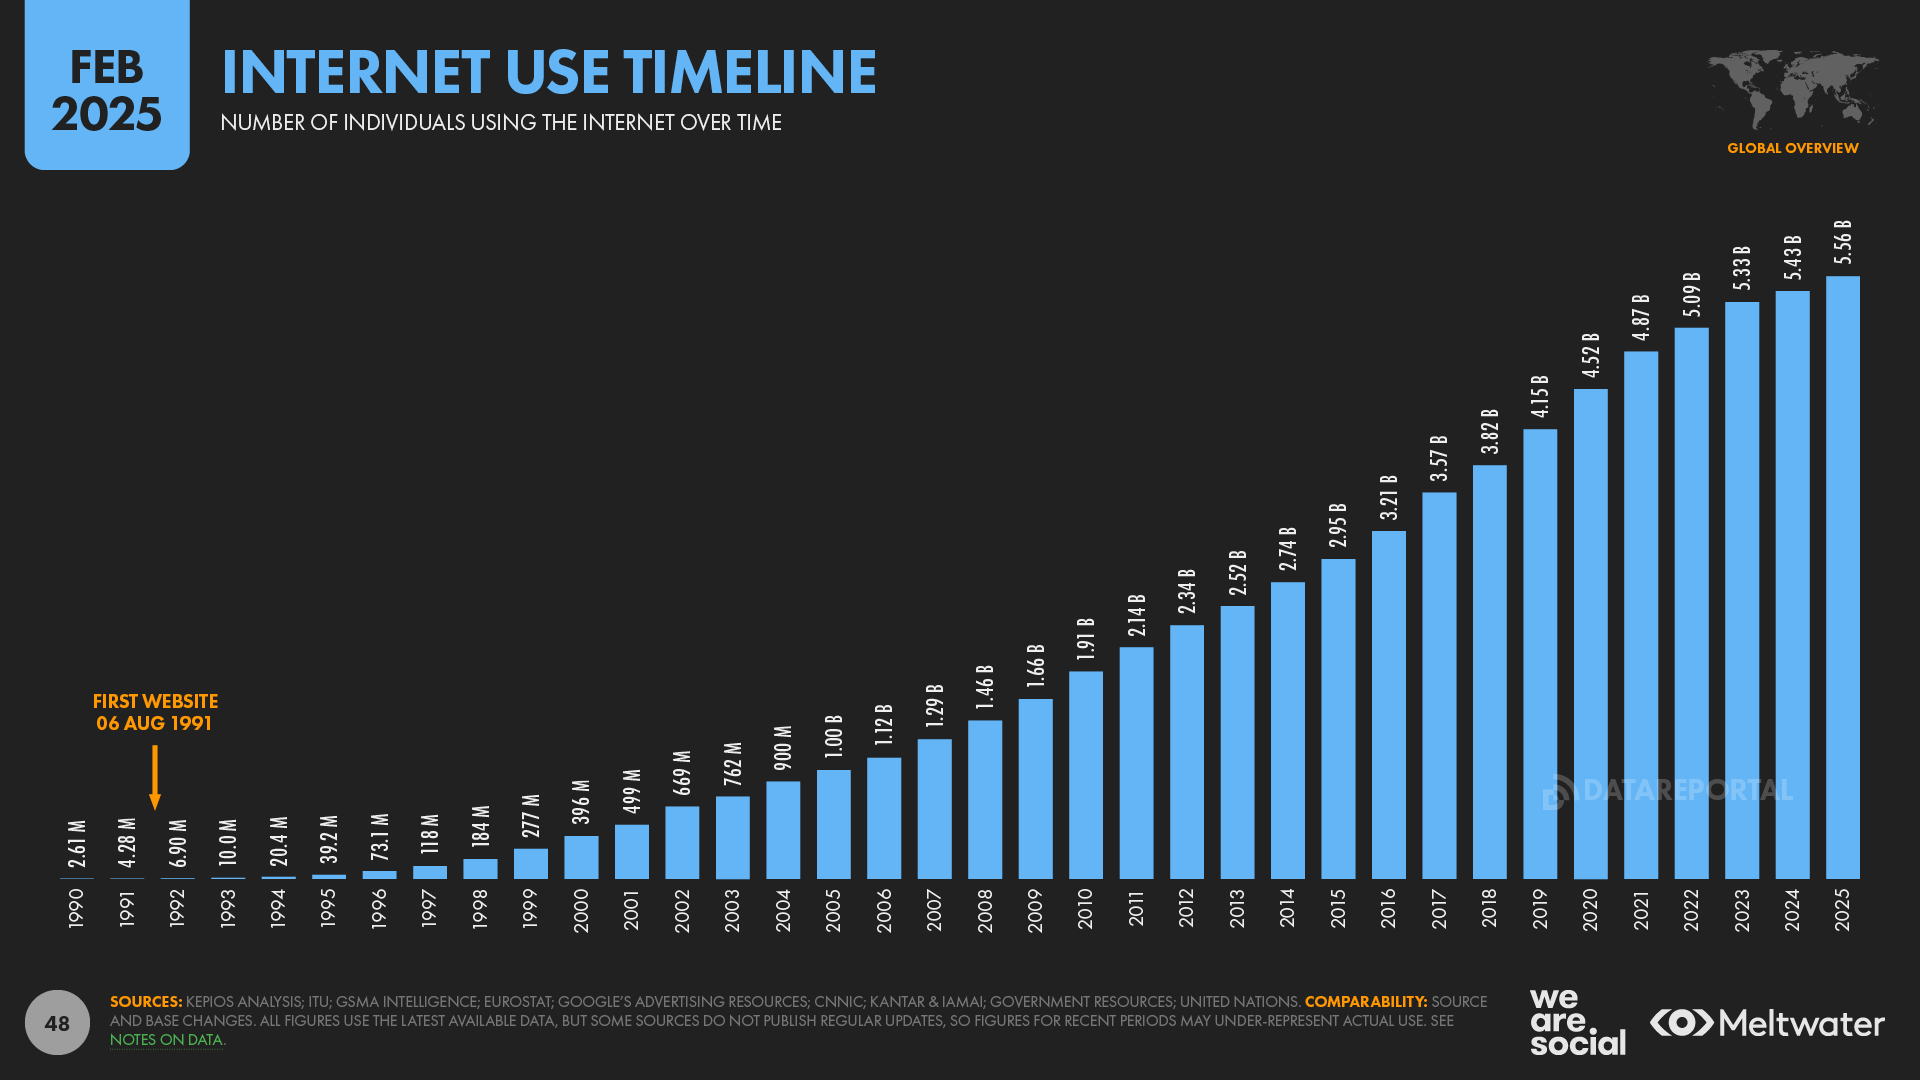
\includegraphics[width=0.8\pagewidth]{../network/internet_users.png}
\end{center}
\end{frame}

\begin{frame}{}
\begin{center}
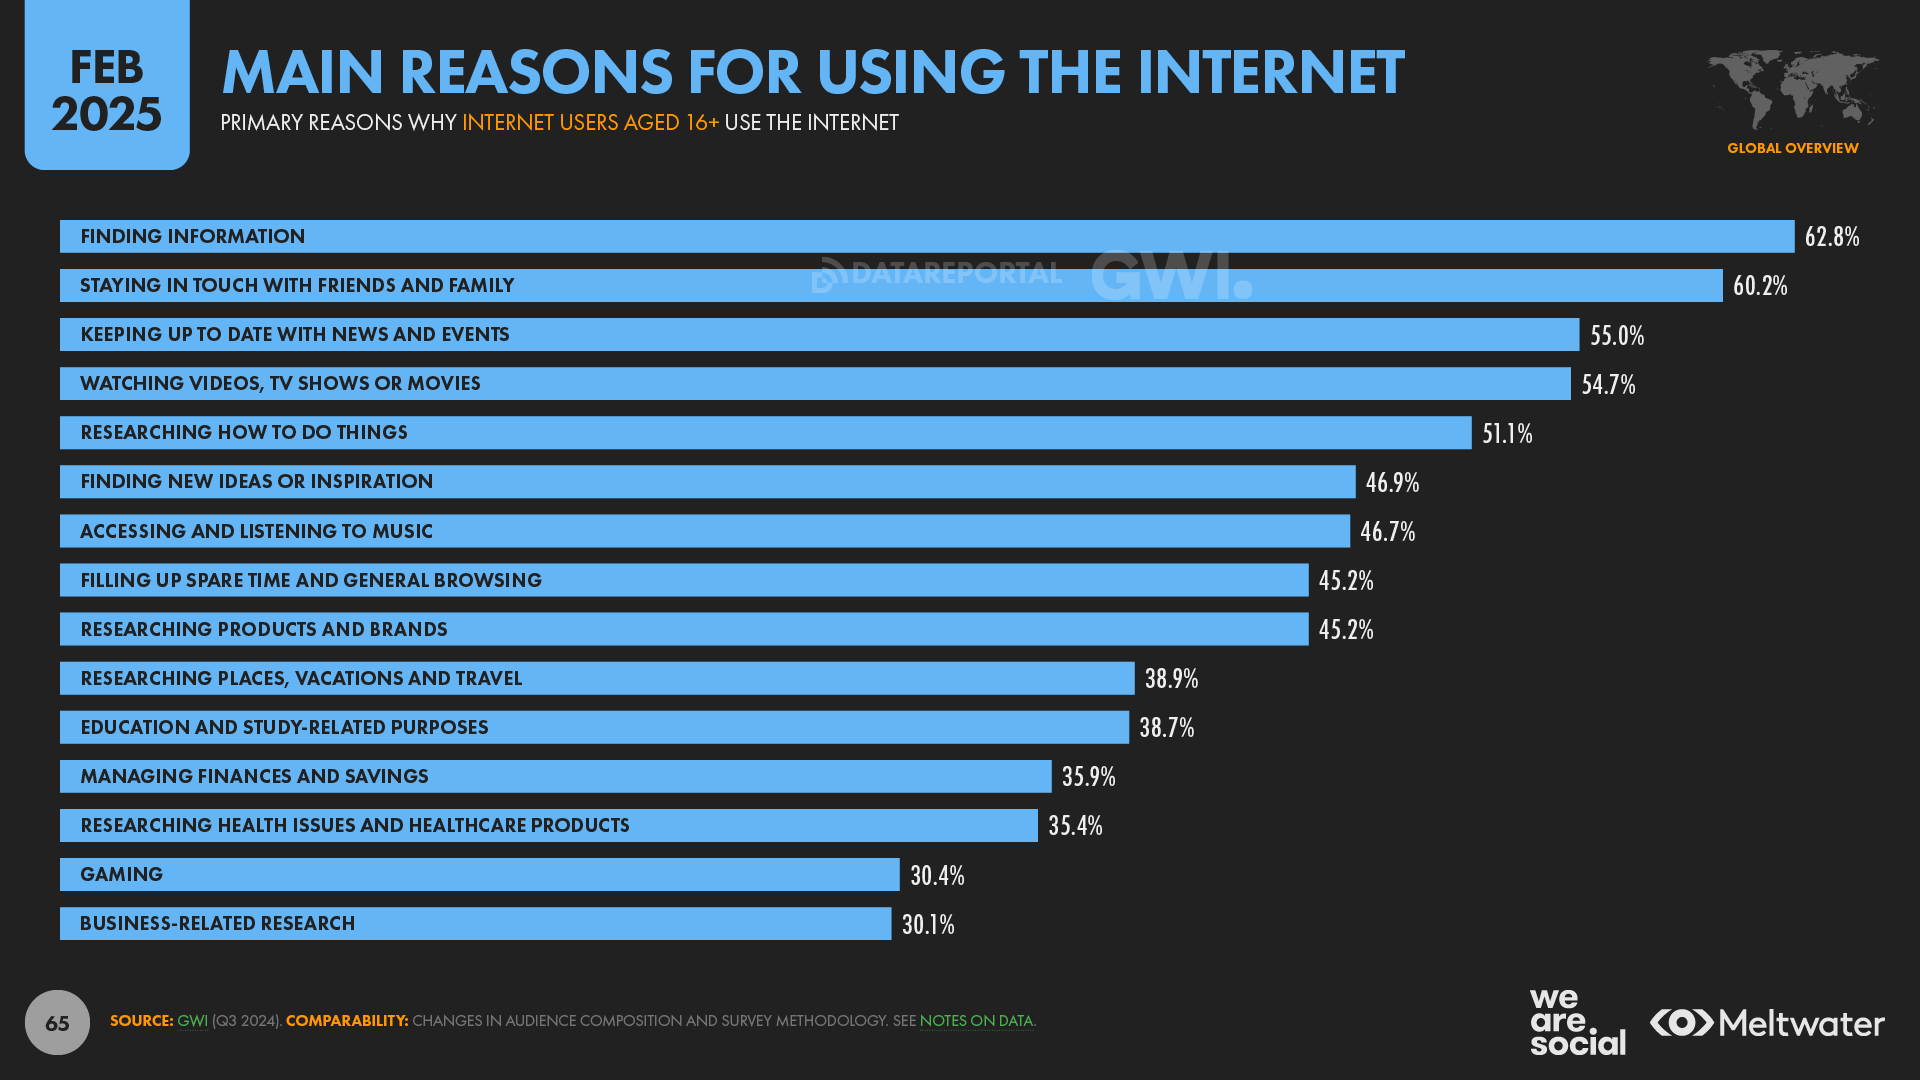
\includegraphics[width=0.8\pagewidth]{../network/internet_reasons.png}
\end{center}
\end{frame}

\begin{frame}{}
\begin{center}
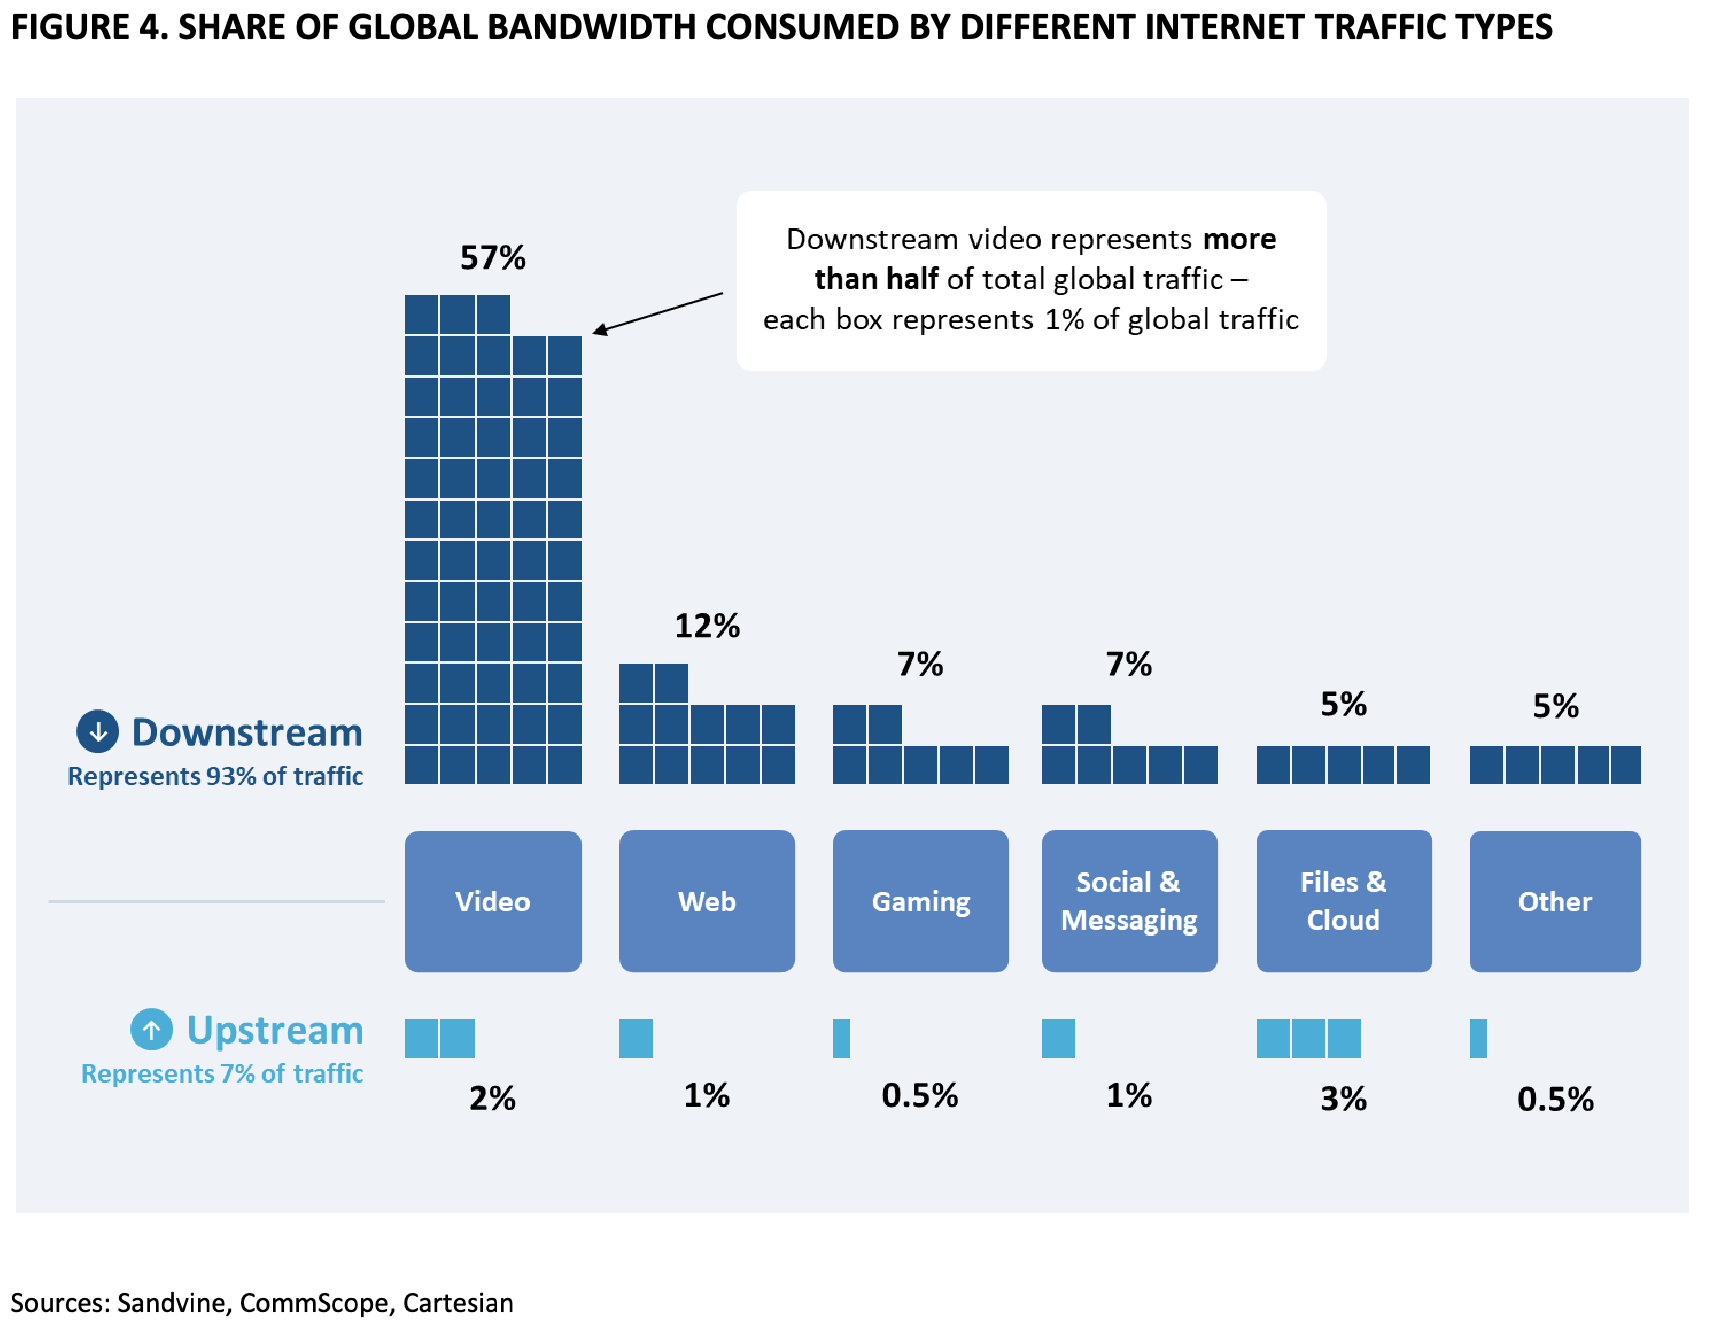
\includegraphics[width=0.8\pagewidth]{../network/internet_data.png}
\end{center}
\end{frame}

\section{ethernet / 802.11 / \ldots}
\begin{frame}{the link layer}
\begin{itemize}
\item Ethernet, Wi-Fi, Bluetooth, DOCSIS (cable modems), \ldots
\vspace{.5cm}
\item allows send/recv messages to machines on \myemph<2>{``same'' network segment}
    \begin{itemize}
    \item typically: wireless range+channel or connected to a single switch/router
    \item could be larger (if \textit{bridging} multiple network segments)
    \item could be smaller (switch/router uses ``virtual LANs'')
    \end{itemize}
\item typically: source+destination specified with MAC addresses
    \begin{itemize}
    \item MAC = media access control
    \item usually manufacturer assigned / hard-coded into device
    \item unique address per port/wifi transmitter/etc.
    \end{itemize}
\item can specify destination of ``anyone'' (called \textit{broadcast})
\item messages usually called ``frames''
\end{itemize}
\end{frame}

\begin{frame}{link layer jobs}
    \begin{itemize}
    \item divide raw bits into messages
    \item identify who message is for on shared radio/wire
    \item handle if two+ machines use radio/wire at same time
    \item drop/resend messages if corruption detected
        \begin{itemize}
        \item resending more common in radio schemes (wifi, etc.)
        \end{itemize}
    \end{itemize}
\end{frame}


\subsection{exercise: why resend?}
\begin{frame}{link layer reliablity?}
    \begin{itemize}
    \item Ethernet + Wifi have checksums
    \vspace{.5cm}
    \item Q1: Why doesn't this give us uncorrupted messages?
        \begin{itemize}
        \item Why do we still have checksums at the higher layers?
        \end{itemize}
    \item Q2: What's a benefit of doing this if we're also doing it in the higher layer?
    \end{itemize}
\end{frame}



\subsection{link layer quality-of-service}

\begin{frame}{link layer quality of service}
if frame gets\ldots \\
\small
\begin{tabular}{l|l|l}
event & on Ethernet & on WiFi \\\hline
collides with another & detected + may resend & resend\\
not received & lose silently & resent \\
header corrupted & usually discard silently & usually resend \\
data corrupted & usually discard silently & usually resend \\
too long & not allowed to send & not allowed to send \\
reordered (v. other messages)  & received out of order & received out of order \\
destination unknown & lose silently & usually resend?? \\
too much being sent & discard excess? & discard excess? \\
\end{tabular}
\end{frame}


\subsection{network layer quality-of-service}

\begin{frame}[fragile]{network layer quality of service}
if packet \ldots \\
\small
\begin{tabular}{l|p{12cm}}
event & on IPv4/v6 \\\hline
collides with another & out of scope --- handled by link layer \\
\myemph<2>{not received}\tikzmark{not recv} & lost silently \\
header corrupted & usually discarded silently \\
data corrupted & received corrupted \\
too long & dropped with notice or ``fragmented'' + recombined \\
reordered (v. other messages) & received out of order \\
destination unknown & usually dropped with notice \\
too much being sent & discard excess \\
\end{tabular}
\begin{tikzpicture}[overlay,remember picture]
\begin{visibleenv}<2>
\node[align=left,my callout=not recv,anchor=north west] at ([xshift=0cm,yshift=-3cm]pic cs:not recv) {
    includes dropped by link layer \\
    (e.g. if detected corrupted there)
};
\end{visibleenv}
\end{tikzpicture}
\end{frame}


\section{firewalls} % FIXME: complete
\begin{frame}{firewalls}
    \begin{itemize}
    \item don't want to expose network service to everyone?
    \item solutions:
        \begin{itemize}
        \item service picky about who it accepts connections from
        \item filters in OS on machine with services
        \item filters on router
        \end{itemize}
    \item later two called ``firewalls''
    \end{itemize}
\end{frame}

\begin{frame}{firewall rules examples?}
    \begin{itemize}
    \item ALLOW tcp port 443 (https) FROM everyone
    \item ALLOW tcp port 22 (ssh) FROM \myemph{my desktop's IP address}
    \item BLOCK tcp port 22 (ssh) FROM everyone else
    \item ALLOW from address X to address Y
    \item \ldots
    \end{itemize}
\end{frame}



\subsection{aside: TCP state machine}
\begin{frame}{TCP state machine}
\begin{itemize}
\item TIME\_WAIT, ESTABLISHED, \ldots?
\vspace{.5cm}
\item OS tracks ``state'' of TCP connection
    \begin{itemize}
    \item am I just starting the connection?
    \item is other end ready to get data?
    \item am I trying to close the connection?
    \item do I need to resend something?
    \end{itemize}
\item standardized set of state names
\end{itemize}
\end{frame}


\begin{frame}{TIME\_WAIT}
\begin{itemize}
\item remember delayed messages?
\vspace{.5cm}
\item problem for TCP ports
\item if I reuse port number, I can get message from old connection
\item solution: TIME\_WAIT to make sure connection really done
    \begin{itemize}
    \item done after sending last message in connection
    \end{itemize}
\end{itemize}
\end{frame}
 % FIXME: diagram
\subsection{DIG trace}

\begin{frame}[fragile]{querying the root}
\begin{Verbatim}[fontsize=\scriptsize]
$ dig @a.root-servers.net www.cs.virginia.edu
...
edu.			172800	IN	NS	b.edu-servers.net.
edu.			172800	IN	NS	f.edu-servers.net.
edu.			172800	IN	NS	i.edu-servers.net.
edu.			172800	IN	NS	a.edu-servers.net.
...
b.edu-servers.net.	172800	IN	A	192.33.14.30
b.edu-servers.net.	172800	IN	AAAA	2001:503:231d::2:30
f.edu-servers.net.	172800	IN	A	192.35.51.30
f.edu-servers.net.	172800	IN	AAAA	2001:503:d414::30
...
\end{Verbatim}
\end{frame}

\begin{frame}[fragile]{querying the edu}
\begin{Verbatim}[fontsize=\scriptsize]
$ dig @b.edu-servers.net www.cs.virginia.edu
...
;; AUTHORITY SECTION:
virginia.edu.		172800	IN	NS	nom.virginia.edu.
virginia.edu.		172800	IN	NS	uvaarpa.virginia.edu.
virginia.edu.		172800	IN	NS	eip-01-aws.net.virginia.edu.

;; ADDITIONAL SECTION:
nom.virginia.edu.	172800	IN	A	128.143.107.101
uvaarpa.virginia.edu.	172800	IN	A	128.143.107.117
eip-01-aws.net.virginia.edu. 172800 IN	A	44.234.207.10
\end{Verbatim}
\end{frame}
\begin{frame}[fragile]{querying virginia.edu}
\begin{Verbatim}[fontsize=\scriptsize]
$ dig @nom.virginia.edu www.cs.virginia.edu
...
;; AUTHORITY SECTION:
cs.virginia.edu.	3600	IN	NS	coresrv01.cs.virginia.edu.

;; ADDITIONAL SECTION:
coresrv01.cs.virginia.edu. 3600	IN	A	128.143.67.11
\end{Verbatim}
\end{frame}

\begin{frame}[fragile]{querying cs.virginia.edu}
\begin{Verbatim}[fontsize=\scriptsize]
$ dig @coresrv01.cs.virginia.edu
...
;; ANSWER SECTION:
www.cs.Virginia.EDU.	172800	IN	A	128.143.67.11

;; AUTHORITY SECTION:
cs.Virginia.EDU.	172800	IN	NS	coresrv01.cs.Virginia.EDU.
...
\end{Verbatim}
\end{frame}

\begin{frame}[fragile]{querying typical ISP's resolver}
\begin{Verbatim}[fontsize=\scriptsize]
$ dig www.cs.virginia.edu
...
;; ANSWER SECTION:
www.cs.Virginia.EDU.	  7183	IN	A	128.143.67.11
..
\end{Verbatim}
\begin{itemize}
\item cached response
\item valid for 7183  more seconds
\item after that everyone needs to check again
\end{itemize}
\end{frame}


\subsection{UDP sockets}
\begin{frame}[fragile]{UDP sockets on IPv4}
\begin{lstlisting}[language=C++,style=smaller]
int fd = socket(AF_INET, SOCK_DGRAM, 0);
struct sockaddr_in my_addr= ...;
bind(fd, &my_addr, sizeof(my_addr))
...
struct sockaddr_in to_addr = ...;
sendto(fd, data, data_size, 0 /* flags */,
    &to_addr, sizeof(to_addr));
struct sockaddr_in from_addr = ...;
recvfrom(fd, &buffer[0], buffer_size, 0,
    &from_addr, sizeof(from_addr));
...
/* or connect() to set default sendto address
\end{lstlisting}
\end{frame}


\subsection{ARP / IPv6 ND routing}

\begin{frame}{what about non-local machines?}
    \begin{itemize}
    \item when configuring network specify:
    \vspace{.5cm}
    \item range of addresses to expect on local network 
        \begin{itemize}
        \item 128.148.67.0-128.148.67.255 on my desktop
        \item ``netmask''
        \end{itemize}
    \item \textit{gateway} machine to send to for things outside my local network
        \begin{itemize}
        \item 128.143.67.1 on my desktop
        \item my desktop looks up the corresponding MAC address
        \end{itemize}
    \end{itemize}
\end{frame}

\begin{frame}[fragile]{routes on my desktop}
\begin{Verbatim}[fontsize=\fontsize{9}{10}\selectfont]
$ /sbin/route -n
Kernel IP routing table
Destination     Gateway         Genmask         Flags Metric Ref    Use Iface
0.0.0.0         128.143.67.1    0.0.0.0         UG    100    0        0 enp0s31f6
128.143.67.0    0.0.0.0         255.255.255.0   U     100    0        0 enp0s31f6
169.254.0.0     0.0.0.0         255.255.0.0     U     1000   0        0 enp0s31f6
\end{Verbatim}
\begin{itemize}
\item network configuration says:
\vspace{.5cm}
\item (line 2) to get to 128.143.67.0--128.143.67.255, send directly on local network
    \begin{itemize}
    \item ``genmask'' is mask (for bitwise operations) to specify how big range is
    \end{itemize}
\item (line 3) to get to 169.254.0.0--169.254.255.255, send directly on local network
\item (line 1) to get anywhere else, use ``gateway'' 128.143.67.1
\end{itemize}
\end{frame}


\subsection{ARP / IPv6 ND}
\againframe<3>{nameAndAddr}
\begin{frame}{two types of addresses?}
    \begin{itemize}
    \item MAC addreses: on link layer
    \item IP addresses: on network layer
    \vspace{.5cm}
    \item how do we know which MAC address to use?
    \end{itemize}
\end{frame}

\begin{frame}[fragile]{a table on my desktop}
my desktop: \\
\begin{Verbatim}[fontsize=\fontsize{9}{10}\selectfont]
$ arp -an
? (128.143.67.140) at 3c:e1:a1:18:bd:5f [ether] on enp0s31f6
? (128.143.67.236) at <incomplete> on enp0s31f6
? (128.143.67.11) at 30:e1:71:5f:39:10 [ether] on enp0s31f6
? (128.143.67.92) at <incomplete> on enp0s31f6
? (128.143.67.5) at d4:be:d9:b0:99:d1 [ether] on enp0s31f6
\end{Verbatim}
\ldots
\end{frame}

\begin{frame}{how is that table made?}
    \begin{itemize}
    \item ask machines on local network (same switch)
    \item ``Who has 128.148.67.140''
    \item the correct one replies
    \end{itemize}
\end{frame}

\begin{frame}{what about non-local machines?}
    \begin{itemize}
    \item when configuring network specify:
    \vspace{.5cm}
    \item range of addresses to expect on local network 
        \begin{itemize}
        \item 128.148.67.0-128.148.67.255 on my desktop
        \item ``netmask''
        \end{itemize}
    \item \textit{gateway} machine to send to for things outside my local network
        \begin{itemize}
        \item 128.143.67.1 on my desktop
        \item my desktop looks up the corresponding MAC address
        \end{itemize}
    \end{itemize}
\end{frame}

\begin{frame}[fragile]{routes on my desktop}
\begin{Verbatim}[fontsize=\fontsize{9}{10}\selectfont]
$ /sbin/route -n
Kernel IP routing table
Destination     Gateway         Genmask         Flags Metric Ref    Use Iface
0.0.0.0         128.143.67.1    0.0.0.0         UG    100    0        0 enp0s31f6
128.143.67.0    0.0.0.0         255.255.255.0   U     100    0        0 enp0s31f6
169.254.0.0     0.0.0.0         255.255.0.0     U     1000   0        0 enp0s31f6
\end{Verbatim}
\begin{itemize}
\item network configuration says:
\vspace{.5cm}
\item (line 2) to get to 128.143.67.0--128.143.67.255, send directly on local network
    \begin{itemize}
    \item ``genmask'' is mask (for bitwise operations) to specify how big range is
    \end{itemize}
\item (line 3) to get to 169.254.0.0--169.254.255.255, send directly on local network
\item (line 1) to get anywhere else, use ``gateway'' 128.143.67.1
\end{itemize}
\end{frame}


% FIXME: HTTP request/response?
\section{and HTTP? (exercise)}
\begin{frame}[fragile]{URLs and HTTP (1)}
\begin{itemize}
    \item \texttt{http://www.foo.com:80/foo/bar?quux\myemph<2>{\#q1}}
    \item lookup IP address of www.foo.com
    \item connect via TCP to port 80:
\end{itemize}
\providecommand{\emphThree}[1]{\myemph<3>{#1}}
\begin{Verbatim}[commandchars=X()]
GET /foo/bar?quux HTTP/1.1
Host: XemphThree(www.foo.com:80)
\end{Verbatim}
\begin{itemize}
    \item<3-> exercise: why include the Host there?
\end{itemize}
\end{frame}



% FIXME: DNS dig example
\subsection{DNS: dig +trace}

\begin{frame}[fragile]{querying the root}
\begin{Verbatim}[fontsize=\scriptsize]
$ dig @a.root-servers.net www.cs.virginia.edu
...
edu.			172800	IN	NS	b.edu-servers.net.
edu.			172800	IN	NS	f.edu-servers.net.
edu.			172800	IN	NS	i.edu-servers.net.
edu.			172800	IN	NS	a.edu-servers.net.
...
b.edu-servers.net.	172800	IN	A	192.33.14.30
b.edu-servers.net.	172800	IN	AAAA	2001:503:231d::2:30
f.edu-servers.net.	172800	IN	A	192.35.51.30
f.edu-servers.net.	172800	IN	AAAA	2001:503:d414::30
...
\end{Verbatim}
\end{frame}

\begin{frame}[fragile]{querying the edu}
\begin{Verbatim}[fontsize=\scriptsize]
$ dig @b.edu-servers.net www.cs.virginia.edu
...
;; AUTHORITY SECTION:
virginia.edu.		172800	IN	NS	nom.virginia.edu.
virginia.edu.		172800	IN	NS	uvaarpa.virginia.edu.
virginia.edu.		172800	IN	NS	eip-01-aws.net.virginia.edu.

;; ADDITIONAL SECTION:
nom.virginia.edu.	172800	IN	A	128.143.107.101
uvaarpa.virginia.edu.	172800	IN	A	128.143.107.117
eip-01-aws.net.virginia.edu. 172800 IN	A	44.234.207.10
\end{Verbatim}
\end{frame}
\begin{frame}[fragile]{querying virginia.edu}
\begin{Verbatim}[fontsize=\scriptsize]
$ dig @nom.virginia.edu www.cs.virginia.edu
...
;; AUTHORITY SECTION:
cs.virginia.edu.	3600	IN	NS	coresrv01.cs.virginia.edu.

;; ADDITIONAL SECTION:
coresrv01.cs.virginia.edu. 3600	IN	A	128.143.67.11
\end{Verbatim}
\end{frame}

\begin{frame}[fragile]{querying cs.virginia.edu}
\begin{Verbatim}[fontsize=\scriptsize]
$ dig @coresrv01.cs.virginia.edu
...
;; ANSWER SECTION:
www.cs.Virginia.EDU.	172800	IN	A	128.143.67.11

;; AUTHORITY SECTION:
cs.Virginia.EDU.	172800	IN	NS	coresrv01.cs.Virginia.EDU.
...
\end{Verbatim}
\end{frame}

\begin{frame}[fragile]{querying typical ISP's resolver}
\begin{Verbatim}[fontsize=\scriptsize]
$ dig www.cs.virginia.edu
...
;; ANSWER SECTION:
www.cs.Virginia.EDU.	  7183	IN	A	128.143.67.11
..
\end{Verbatim}
\begin{itemize}
\item cached response
\item valid for 7183  more seconds
\item after that everyone needs to check again
\end{itemize}
\end{frame}


\section{spoofing?}
\begin{frame}{spoofing}
    \begin{itemize}
    \item if I only allow connections from my desktop's IP addresses, \\
        how would you attack this?
    \vspace{.5cm}
    \item hint: how do we know what address messages come from?
    \end{itemize}
\end{frame}



\subsection{example: echo client/server}
\subsubsection{server setup}
\begin{frame}[fragile,label=connSetupServer]{connection setup: server, manual}
\begin{lstlisting}[
    language=C++,style=smaller,
    moredelim={**[is][\btHL<2|handout:2>]{@2}{2@}},
    moredelim={**[is][\btHL<3|handout:3>]{@3}{3@}},
    moredelim={**[is][\btHL<4|handout:4>]{@4}{4@}},
    moredelim={**[is][\btHL<5|handout:5>]{@5}{5@}},
    moredelim={**[is][\btHL<6|handout:6>]{@6}{6@}},
]
int server_socket_fd = socket(AF_INET, SOCK_STREAM, IPPROTO_TCP);
struct sockaddr_in addr;
addr.sin_family = AF_INET;
addr.sin_addr.s_addr = @2INADDR_ANY2@; /* "any address I can use" */
    @3/* or: addr.s_addr.in_addr = INADDR_LOOPBACK (127.0.0.1) */3@
    /* or: addr.s_addr.in_addr = htonl(...); */
addr.sin_port = @4htons(9999)4@; /* port number 9999 */

if (bind(server_socket_fd, &addr, sizeof(addr)) < 0) {
    /* handle error */
}
listen(server_socket_fd, @4MAX_NUM_WAITING4@);
...
int socket_fd = accept(server_socket_fd, NULL);
\end{lstlisting}
\begin{tikzpicture}[overlay,remember picture]
\tikzset{
    box/.style={draw=red, ultra thick,fill=white,at={([yshift=-2cm]current page.north)},anchor=north,align=left},
    box low/.style={draw=red, ultra thick,fill=white,at={([yshift=-6cm]current page.north)},anchor=north,align=left},
}
\begin{visibleenv}<2>
\node[box low] {
    INADDR\_ANY: accept connections for any address I can! \\
    alternative: specify specific address
};
\end{visibleenv}
\begin{visibleenv}<3>
\node[box low] {
    bind to 127.0.0.1? only accept connections \myemph{from same machine} \\
    what we recommend for FTP server assignment
};
\end{visibleenv}
\begin{visibleenv}<4>
\node[box low] {
    choose the number of unaccepted connections
};
\end{visibleenv}
\end{tikzpicture}
\end{frame}

\subsubsection{client setup}
\begin{frame}[fragile,label=connSetupClientManual]{connection setup: client --- manual addresses}
\begin{lstlisting}[
    language=C++,style=smaller,
    moredelim={**[is][\btHL<1|handout:1>]{@1}{1@}},
    moredelim={**[is][\btHL<2|handout:2>]{@2}{2@}},
    moredelim={**[is][\btHL<3|handout:3>]{@3}{3@}},
    moredelim={**[is][\btHL<4|handout:4>]{@4}{4@}},
    moredelim={**[is][\btHL<5|handout:5>]{@5}{5@}},
    moredelim={**[is][\btHL<6|handout:6>]{@6}{6@}},
]
int sock_fd;

server = /* code on later slide */;
sock_fd = @1socket1@(
    @2AF_INET2@, /* IPv4 */
    @2SOCK_STREAM2@, /* byte-oriented */
    @2IPPROTO_TCP2@
);
if (sock_fd < 0) { /* handle error */ }

@4struct sockaddr_in addr4@;
addr.sin_family = AF_INET;
addr.sin_addr.s_addr = @3htonl3@(2156872459); /* 128.143.67.11 */
addr.sin_port = @3htons3@(80); /* port 80 */
if (@1connect1@(sock_fd, (struct sockaddr*) &addr, sizeof(addr)) {
    /* handle error */
}
DoClientStuff(sock_fd); /* read and write from sock_fd */
close(sock_fd);
\end{lstlisting}
\begin{tikzpicture}[overlay,remember picture]
\tikzset{
    box/.style={draw=red, ultra thick,fill=white,at={([yshift=-2cm]current page.north)},anchor=north,align=left},
    box low/.style={draw=red, ultra thick,fill=white,at={([yshift=-5cm]current page.north)},anchor=north,align=left},
}
\begin{visibleenv}<2>
\node[box low] {
    specify IPv4 instead of IPv6 or local-only sockets \\
    specify TCP (byte-oriented) instead of UDP (`datagram' oriented)
};
\end{visibleenv}
\begin{visibleenv}<3>
\node[box] {
    htonl/s = host-to-network long/short \\
    network byte order = big endian
};
\end{visibleenv}
\begin{visibleenv}<4>
\node[box] {
    struct representing IPv4 address + port number \\
    declared in \lstinline|<netinet/in.h>| \\
    see \texttt{man 7 ip} on Linux for docs
};
\end{visibleenv}
\end{tikzpicture}
\end{frame}


\subsubsection{read/write code}

\begin{frame}[fragile,label=echoClient]{echo client/server}
\begin{lstlisting}[
    language=C++,
    basicstyle=\sourcecodepro\EmptyMapping\fontsize{10}{11}\selectfont,
    keywordstyle=\sourcecodepro\EmptyMapping\fontsize{10}{11}\selectfont,
    moredelim={**[is][\btHL<1|handout:1>]{@1}{1@}},
    moredelim={**[is][\btHL<2|handout:2>]{@2}{2@}},
    moredelim={**[is][\btHL<3|handout:3>]{@3}{3@}},
    moredelim={**[is][\btHL<4|handout:4>]{@4}{4@}},
    moredelim={**[is][\btHL<5|handout:5>]{@5}{5@}},
    moredelim={**[is][\btHL<6|handout:6>]{@6}{6@}},
]
void client_for_connection(int socket_fd) {
    int n; char send_buf[MAX_SIZE]; char recv_buf[MAX_SIZE];
    while (prompt_for_input(send_buf, MAX_SIZE)) {
        n = @2write(socket_fd, send_buf, strlen(send_buf))2@;
        if (n != strlen(send_buf)) {...error?...}
        n = @3read(socket_fd, recv_buf, MAX_SIZE)3@;
        if (n <= 0) return; // error or EOF 
        write(STDOUT_FILENO, recv_buf, n);
    }
}
\end{lstlisting}
\hrule
\begin{lstlisting}[
    language=C++,style=smaller,
    moredelim={**[is][\btHL<1|handout:1>]{@1}{1@}},
    moredelim={**[is][\btHL<2|handout:2>]{@2}{2@}},
    moredelim={**[is][\btHL<3|handout:3>]{@3}{3@}},
    moredelim={**[is][\btHL<4|handout:4>]{@4}{4@}},
    moredelim={**[is][\btHL<5|handout:5>]{@5}{5@}},
    moredelim={**[is][\btHL<6|handout:6>]{@6}{6@}},
]
void server_for_connection(int socket_fd) {
    int read_count, write_count; char request_buf[MAX_SIZE];
    while (1) {
        read_count = @2read(socket_fd, request_buf, MAX_SIZE)2@;
        if (read_count <= 0) return; // error or EOF 
        write_count = @3write(socket_fd, request_buf, read_count)3@;
        if (read_count != write_count) {...error?...}
    }
}
\end{lstlisting}
\end{frame}



\subsection{more normal connection setup}
\begin{frame}[fragile,label=connSetupServerLookup]{connection setup: server, address setup}
\begin{lstlisting}[
    language=C++,style=smaller,
    moredelim={**[is][\btHL<2|handout:2>]{@2}{2@}},
    moredelim={**[is][\btHL<3|handout:3>]{@3}{3@}},
    moredelim={**[is][\btHL<4|handout:4>]{@4}{4@}},
    moredelim={**[is][\btHL<5|handout:5>]{@5}{5@}},
    moredelim={**[is][\btHL<6|handout:6>]{@6}{6@}},
]
/* example (hostname, portname) = ("127.0.0.1", "443") */
const char *@2hostname2@; const char *@3portname3@;
...
struct addrinfo *server;
struct addrinfo hints;
int rv;

memset(&hints, 0, sizeof(hints));
hints.ai_family = AF_INET; /* for IPv4 */
/* or: */ hints.ai_family = AF_INET6; /* for IPv6 */
/* or: */ hints.ai_family = AF_UNSPEC; /* I don't care */
@4hints.ai_flags = AI_PASSIVE4@;

rv = getaddrinfo(hostname, portname, &hints, &server);
if (rv != 0) { /* handle error */ }
\end{lstlisting}
\begin{tikzpicture}[overlay,remember picture]
\tikzset{
    box/.style={draw=red, ultra thick,fill=white,at={([yshift=-2cm]current page.north)},anchor=north,align=left},
    box low/.style={draw=red, ultra thick,fill=white,at={([yshift=-6cm]current page.north)},anchor=north,align=left},
}
\begin{visibleenv}<2>
\node[box low] {
    \texttt{hostname} could also be NULL \\
    means ``use all possible addresses'' \\
    only makes sense for servers
};
\end{visibleenv}
\begin{visibleenv}<3>
\node[box low] {
    \texttt{portname} could also be NULL \\
    means ``choose a port number for me'' \\
    only makes sense for servers
};
\end{visibleenv}
\begin{visibleenv}<4>
\node[box] {
    AI\_PASSIVE: ``I'm going to use bind''
};
\end{visibleenv}
\end{tikzpicture}
\end{frame}


\begin{frame}[fragile,label=connSetupServerAddrinfo]{connection setup: server, addrinfo}
\begin{lstlisting}[
    language=C++,style=smaller,
    moredelim={**[is][\btHL<2|handout:2>]{@2}{2@}},
    moredelim={**[is][\btHL<3|handout:3>]{@3}{3@}},
    moredelim={**[is][\btHL<4|handout:4>]{@4}{4@}},
    moredelim={**[is][\btHL<5|handout:5>]{@5}{5@}},
    moredelim={**[is][\btHL<6|handout:6>]{@6}{6@}},
]
struct addrinfo *server;
... getaddrinfo(...) ...

int server_socket_fd = socket(
    server->ai_family,
    server->ai_sockttype,
    server->ai_protocol
);

if (bind(server_socket_fd, ai->ai_addr, ai->ai_addr_len)) < 0) {
    /* handle error */
}
listen(server_socket_fd, MAX_NUM_WAITING);
...
int socket_fd = accept(server_socket_fd, NULL);
\end{lstlisting}
\end{frame}


\begin{frame}[fragile,label=connSetupClientAddrInfo]{connection setup: client, using addrinfo}
\begin{lstlisting}[
    language=C++,style=smaller,
    moredelim={**[is][\btHL<2|handout:2>]{@2}{2@}},
    moredelim={**[is][\btHL<3|handout:3>]{@3}{3@}},
    moredelim={**[is][\btHL<4|handout:4>]{@4}{4@}},
    moredelim={**[is][\btHL<5|handout:5>]{@5}{5@}},
    moredelim={**[is][\btHL<6|handout:6>]{@6}{6@}},
]
int sock_fd; 
@2struct addrinfo2@ *server = /* code on next slide */;

sock_fd = socket(
    @3server->ai_family3@,  
     // ai_family = AF_INET (IPv4) or AF_INET6 (IPv6) or ...
    @3server->ai_socktype3@,
     // ai_socktype = SOCK_STREAM (bytes) or ...
    @3server->ai_prototcol3@
     // ai_protocol = IPPROTO_TCP or ...
);
if (sock_fd < 0) { /* handle error */ }
if (connect(sock_fd, server->@4ai_addr4@, server->@4ai_addrlen4@) < 0) {
    /* handle error */
}
@5freeaddrinfo(server);5@
DoClientStuff(sock_fd); /* read and write from sock_fd */
close(sock_fd);
\end{lstlisting}
\begin{tikzpicture}[overlay,remember picture]
\tikzset{
    box/.style={draw=red, ultra thick,fill=white,at={([yshift=-2cm]current page.north)},anchor=north,align=left},
    box low/.style={draw=red, ultra thick,fill=white,at={([yshift=-5cm]current page.north)},anchor=north,align=left},
}
\begin{visibleenv}<2>
\node[box low] {
    addrinfo contains all information needed to setup socket \\
    set by \texttt{getaddrinfo} function (next slide) \\
    handles IPv4 and IPv6 \\
    handles DNS names, service names
};
\end{visibleenv}
\begin{visibleenv}<4>
\node[box] {
    ai\_addr points to struct representing address \\
    type of struct depends whether IPv6 or IPv4
};
\end{visibleenv}
\begin{visibleenv}<5>
\node[box] {
    since addrinfo contains pointers to dynamically allocated memory, \\
    call this function to free everything
};
\end{visibleenv}
\end{tikzpicture}
\end{frame}

\begin{frame}[fragile,label=serverLookupClient]{connection setup: lookup address}
\begin{lstlisting}[
    language=C++,style=smaller,
    moredelim={**[is][\btHL<2|handout:2>]{@2}{2@}},
    moredelim={**[is][\btHL<3|handout:3>]{@3}{3@}},
    moredelim={**[is][\btHL<4|handout:4>]{@4}{4@}},
    moredelim={**[is][\btHL<5|handout:5>]{@5}{5@}},
    moredelim={**[is][\btHL<6|handout:6>]{@6}{6@}},
]
/* example hostname, portname = "www.cs.virginia.edu", "443" */
const char *hostname; const char *portname;
...
struct addrinfo *server;
struct addrinfo hints;
int rv;
memset(&hints, 0, sizeof(hints));
@3hints.ai_family = AF_UNSPEC3@; /* for IPv4 OR IPv6 */
// hints.ai_family = AF_INET4; /* for IPv4 only */

hints.ai_socktype = SOCK_STREAM; /* byte-oriented --- TCP */
rv = getaddrinfo(hostname, portname, &hints, @2&server2@);
if (rv != 0) { /* handle error */ }

/* eventually freeaddrinfo(result) */
\end{lstlisting}
\begin{tikzpicture}[overlay,remember picture]
\tikzset{
    box/.style={draw=red, ultra thick,fill=white,at={([yshift=-2cm]current page.north)},anchor=north,align=left},
    box low/.style={draw=red, ultra thick,fill=white,at={([yshift=-5cm]current page.north)},anchor=north,align=left},
}
\begin{visibleenv}<2>
\node[box low] {
    NB: pass pointer \textit{to pointer} to addrinfo to fill in
};
\end{visibleenv}
\begin{visibleenv}<3>
\node[box] {
    AF\_UNSPEC: choose between IPv4 and IPv6 for me \\
    AF\_INET, AF\_INET6: choose IPv4 or IPV6 respectively
};
\end{visibleenv}
\end{tikzpicture}
\end{frame}


\subsection{other connection setup options}
\begin{frame}[fragile,label=serverLookupClientMulti]{connection setup: multiple server addresses}
\begin{lstlisting}[
    language=C++,style=smaller,
    moredelim={**[is][\btHL<2|handout:2>]{@2}{2@}},
    moredelim={**[is][\btHL<3|handout:3>]{@3}{3@}},
    moredelim={**[is][\btHL<4|handout:4>]{@4}{4@}},
    moredelim={**[is][\btHL<5|handout:5>]{@5}{5@}},
    moredelim={**[is][\btHL<6|handout:6>]{@6}{6@}},
]
struct addrinfo *server;
...
rv = getaddrinfo(hostname, portname, &hints, &server);
if (rv != 0) { /* handle error */ }

for (struct addrinfo *current = server; current != NULL;
      @2current = current->ai_next2@) {
    sock_fd = socket(current->ai_family, current->ai_socktype, current->ai_protocol);
    if (sock_fd < 0) continue;
    if (connect(sock_fd, current->ai_addr, current->ai_addrlen) == 0) {
        break;
    }
    close(sock_fd); // connect failed
}
freeaddrinfo(server);
DoClientStuff(sock_fd);
close(sock_fd);
\end{lstlisting}
\begin{tikzpicture}[overlay,remember picture]
\tikzset{
    box/.style={draw=red, ultra thick,fill=white,at={([yshift=-2cm]current page.north)},anchor=north,align=left},
    box low/.style={draw=red, ultra thick,fill=white,at={([yshift=-6.5cm]current page.north)},anchor=north,align=left},
}
\begin{visibleenv}<2>
\node[box low] {
    addrinfo is a linked list \\
    name can correspond to multiple addresses \\
    example: redundant copies of web server \\
    example: an IPv4 address and IPv6 address \\
    example: wired + wireless connection on one machine
};
\end{visibleenv}
\end{tikzpicture}
\end{frame}

\begin{frame}[fragile,label=serverLookupClientOld]{connection setup: old lookup function}
\begin{lstlisting}[language=C++,style=smaller]
/* example hostname, portnum= "www.cs.virginia.edu", 443*/
const char *hostname; int portnum;
...
struct hostent *server_ip;
server_ip = gethostbyname(hostname);

if (server_ip == NULL) { /* handle error */ }

struct sockaddr_in addr;
addr.s_addr = *(struct in_addr*) server_ip->h_addr_list[0];
addr.sin_port = htons(portnum);
sock_fd = socket(AF_INET, SOCK_STREAM, IPPROTO_TCP);
connect(sock_fd, &addr, sizeof(addr));
...
\end{lstlisting}
\end{frame}

\begin{frame}{aside: on server port numbers}
    \begin{itemize}
    \item Unix convention: must be \texttt{root} to use ports 0--1023
        \begin{itemize}
        \item root = superuser = `adminstrator user' = what sudo does
        \end{itemize}
    \item so, for testing: probably ports $>$ 1023
    \end{itemize}
\end{frame}


